\section{Introduction}
\subsection{Motivation}
The K96 output is affected by the concentration/molar fraction of methane, carbon dioxide and water, as expected. However, the K96 output is also influenced by environmental parameters such as temperature, humidity and pressure. The purpose of the calibration model is to mitigate the unwanted effects of the environmental parameters on the K96 output.\\

In order to train a calibration model in the form of a ML model, a training dataset is required. Furthermore, the training dataset must capture the effects of both the gas molar fraction and the environmental parameters on the K96 output.

\subsection{Previous Studies}\label{sec:previous_studies}
Multiple previous studies has been conducted on the calibration of the K96 using ML, in the following, three of them are be presented, focusing on the data collection.

\subsubsection*{\href{https://ieeexplore.ieee.org/abstract/document/11078940}{Accurate Measurements of Methane, Carbon Dioxide for Arctic and Wetland Conditions using NDIR Technology and AI-based Calibration \cite{11078940}}}

The \textbf{setup} used in the study is presented in Figure \ref{fig:accurate_measurments_setup}. A target gas (methane or carbon dioxide), dry air and humid air are mixed in a mixing chamber. The flow of each gas is controlled, enabling control of the molar fraction and humidity. A temperature coil enables control of the temperature. The mixed gas is ultimately measured by the K96 and a reference instrument.

\begin{figure}[htbp]
    \centering
    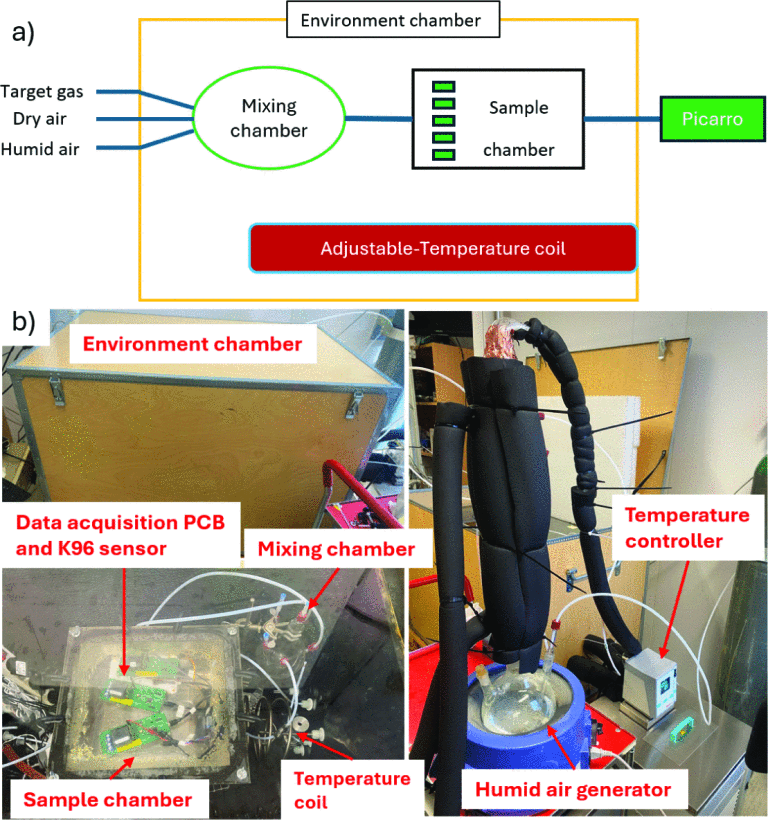
\includegraphics[width=1\linewidth]{figs/accurate_measurments/gia2-p6-gia-large.png}
    \caption{Setup used in reference \cite{11078940}. 
    % a) Theoretical setup. b) Practical setup.
    }
    \label{fig:accurate_measurments_setup}
\end{figure}

\begin{figure}[htbp]
\begin{subfigure}{0.49\textwidth}
    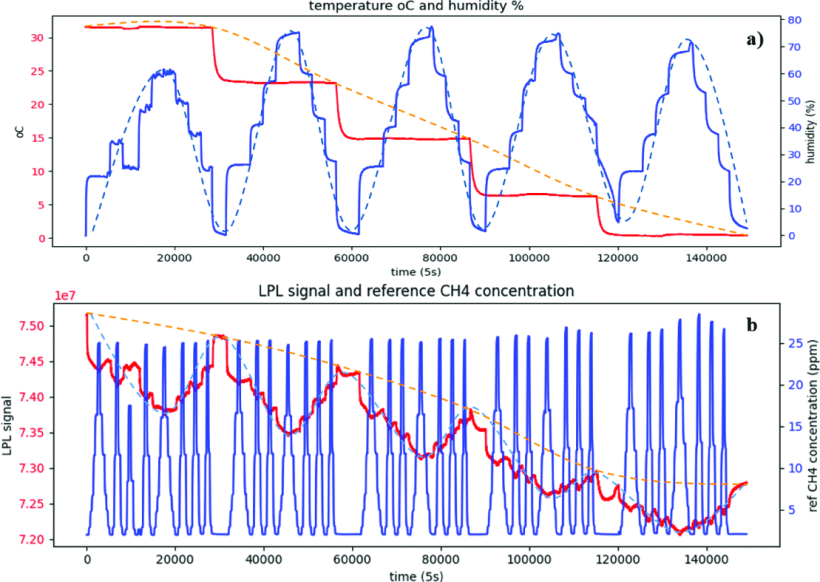
\includegraphics[width=0.9\linewidth]{figs/accurate_measurments/gia3-p6-gia-large.png} 
    \caption{For methane.}
    \label{fig:accurate_measurments_data_ch4}
\end{subfigure}
\begin{subfigure}{0.49\textwidth}
    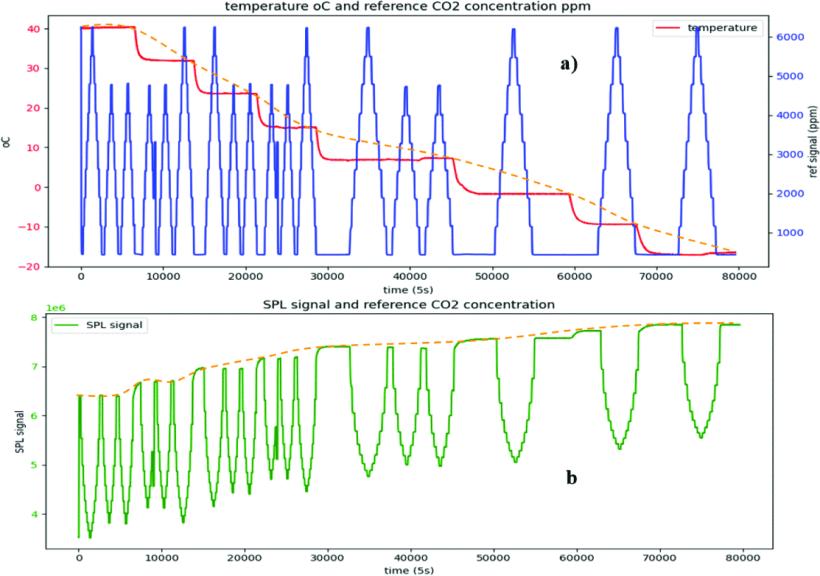
\includegraphics[width=0.9\linewidth]{figs/accurate_measurments/gia4-p6-gia-large.png}
    \caption{For carbon dioxide.}
    \label{fig:accurate_measurments_data_co2}
\end{subfigure}
\caption{Calibration datasets obtained in reference \cite{11078940}.}
\label{fig:accurate_measurments_data}
\end{figure}

The \textbf{calibration dataset}s obtained in the study are presented in Figure \ref{fig:accurate_measurments_data}. For methane, the temperature is varied with the lowest frequency, in steps. At each temperature step, the humidity is varied with a higher frequency, in steps. At each humidity step, the molar fraction is varied with the highest frequency. For carbon dioxide the procedure is the same, but without the variation of humidity.

\subsubsection*{\href{https://www.mdpi.com/1424-8220/25/24/7691}{Machine Learning-Enhanced NDIR Methane Sensing Solution for Robust Outdoor Continuous Monitoring Applications \cite{s25247691}}}

The \textbf{setup} used in the study is presented in Figure \ref{fig:ml_enhanced_setup}. One methane gas line and two nitrogen gas lines are used. One of the nitrogen gas lines is passed through a water bubbler to increase its humidity. The flow of each gas line is controlled, enabling control of the molar fraction and humidity. All gas lines enter a temperature-controlled oven, enabling control of the temperature. Inside the oven, the mixed gas is ultimately measured by the K96 and a reference instrument.

\begin{figure}[htbp]
    \centering
    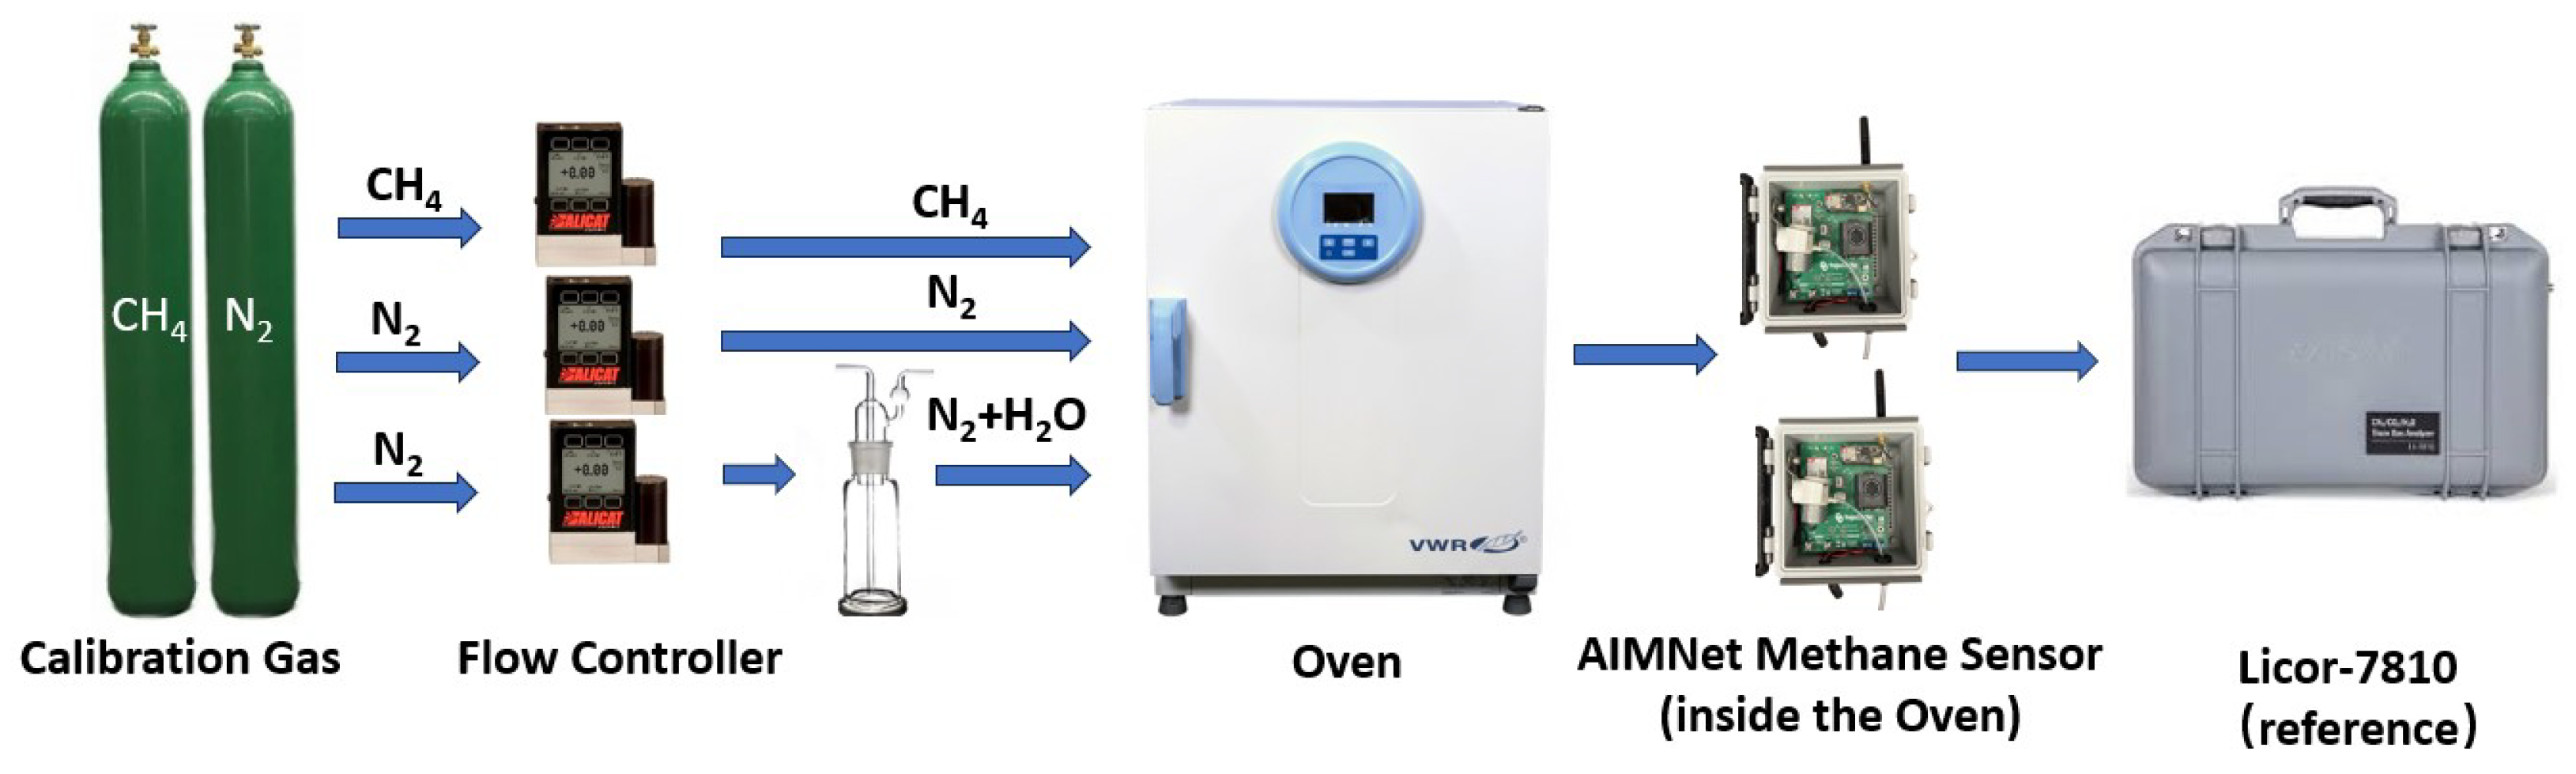
\includegraphics[width=1\linewidth]{figs/ml_enhanced/sensors-25-07691-g003.png}
    \caption{Setup used in reference \cite{s25247691}.}
    \label{fig:ml_enhanced_setup}
\end{figure}

\begin{figure}[htbp]
    \centering
    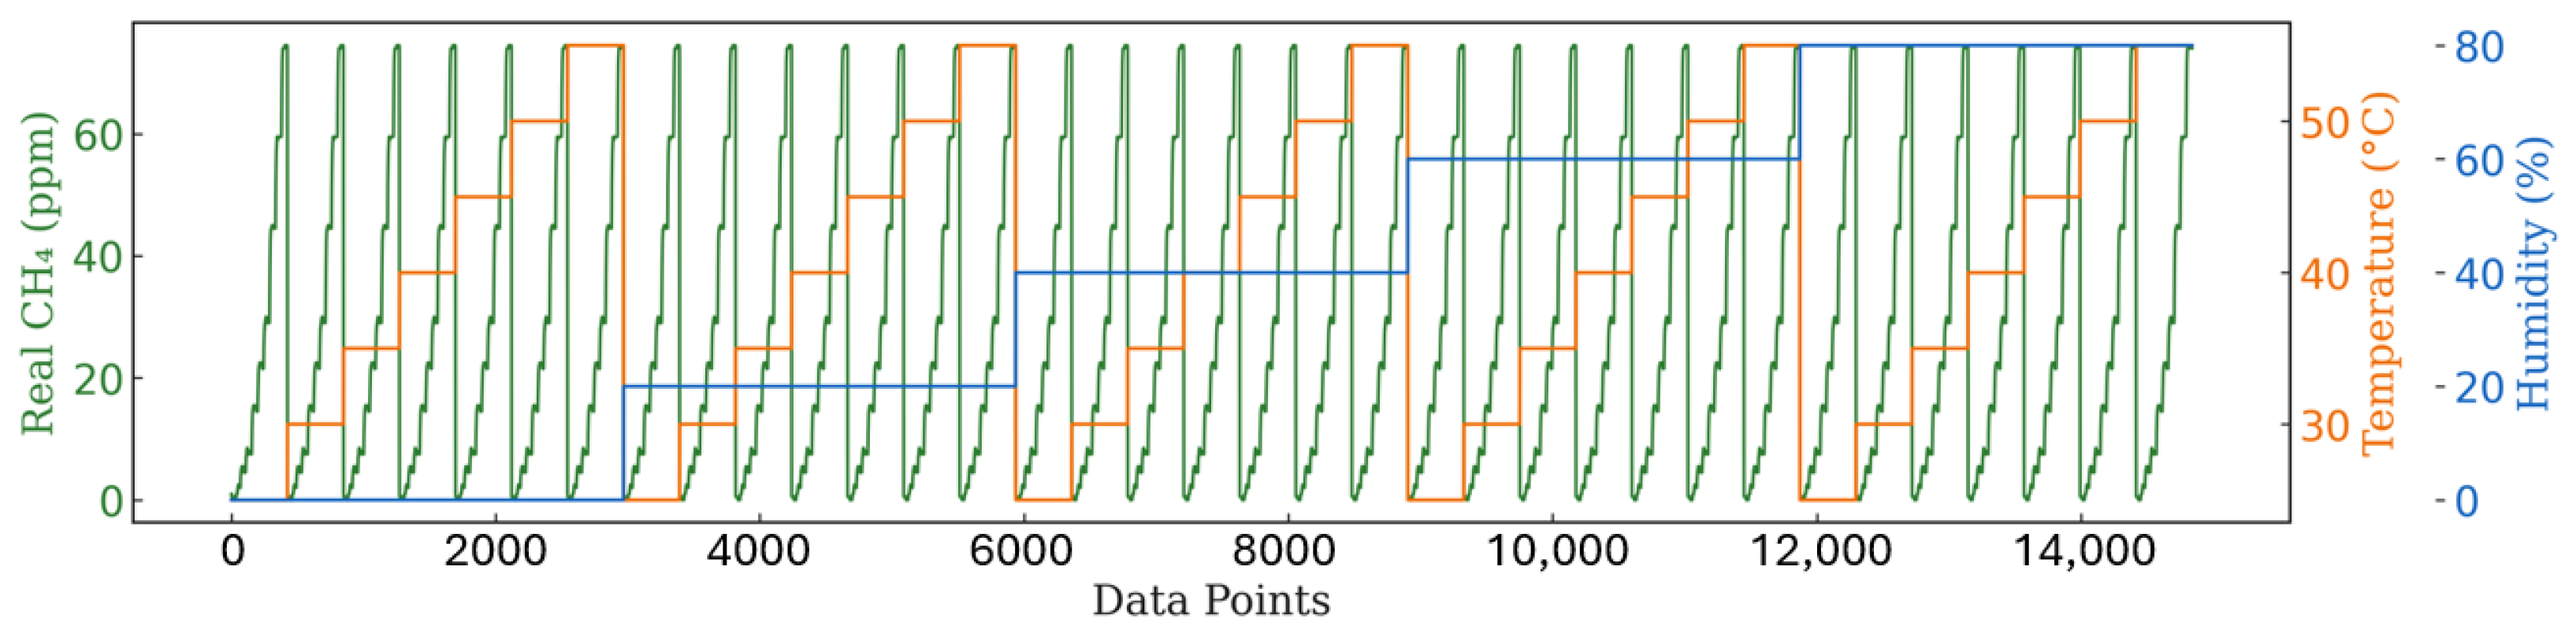
\includegraphics[width=1\linewidth]{figs/ml_enhanced/sensors-25-07691-g004.png}
    \caption{Calibration dataset obtained in reference \cite{s25247691}.}
    \label{fig:ml_enhanced_data}
\end{figure}

The \textbf{calibration dataset} obtained in the study is presented in Figure \ref{fig:ml_enhanced_data}. The humidity is varied with the lowest frequency, in steps. At each humidity step, the temperature is varied with a higher frequency, in steps. At each temperature step, the molar fraction is varied with the highest frequency, allowing several minutes at each step to ensure signal stabilization.

\subsubsection*{\href{http://urn.kb.se/resolve?urn=urn:nbn:se:uu:diva-592179}{Calibration of an NDIR Gas Sensor for Stratospheric Pressure and Temperature Conditions \cite{Olle2078608}}}

The \textbf{setup}s used in the study are presented in Figures \ref{fig:calibration_setup_dry_reference} and \ref{fig:calibration_setup_humid}. The setup for dry and reference instrument data uses a calibration gas (methane and carbon dioxide) and ambient air, respectively. A compressor pressurizes the gas into a pressure chamber covered with a heat blanket, enabling control of the pressure and temperature. Ultimately, the gas is measured by the K96, in the pressure chamber. The setup for humid data is the same, but with a dew point generator upstream of the compressor, enabling the control of the humidity.

\begin{figure}[htbp]
\begin{subfigure}{0.49\textwidth}
    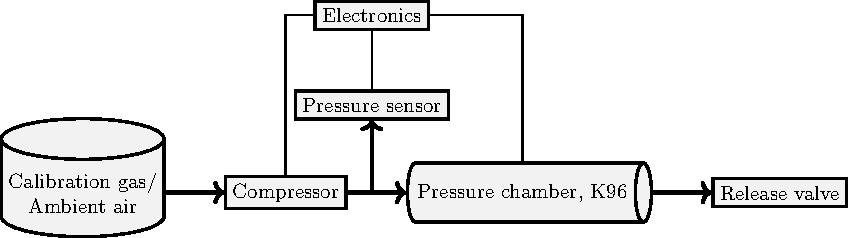
\includegraphics[width=0.9\linewidth]{figs/calibration/dry_reference_setup.pdf} 
    \caption{{\footnotesize For dry and reference instrument data}.}
    \label{fig:calibration_setup_dry_reference}
\end{subfigure}
\begin{subfigure}{0.49\textwidth}
    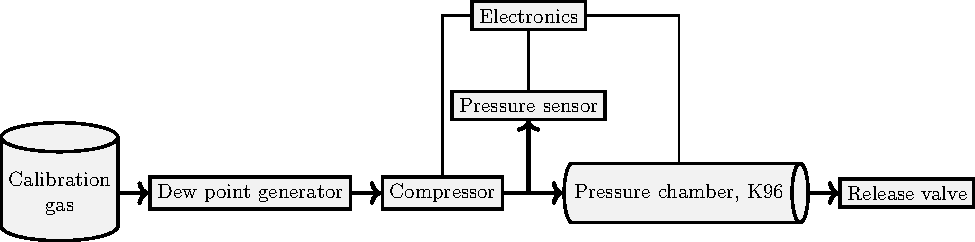
\includegraphics[width=0.9\linewidth]{figs/calibration/humid_setup.pdf} 
    \caption{For humid data.}
    \label{fig:calibration_setup_humid}
\end{subfigure}
\caption{Setups used in reference \cite{Olle2078608}.}
\label{fig:calibration_setup}
\end{figure}

\begin{figure}[htbp]
    \centering
    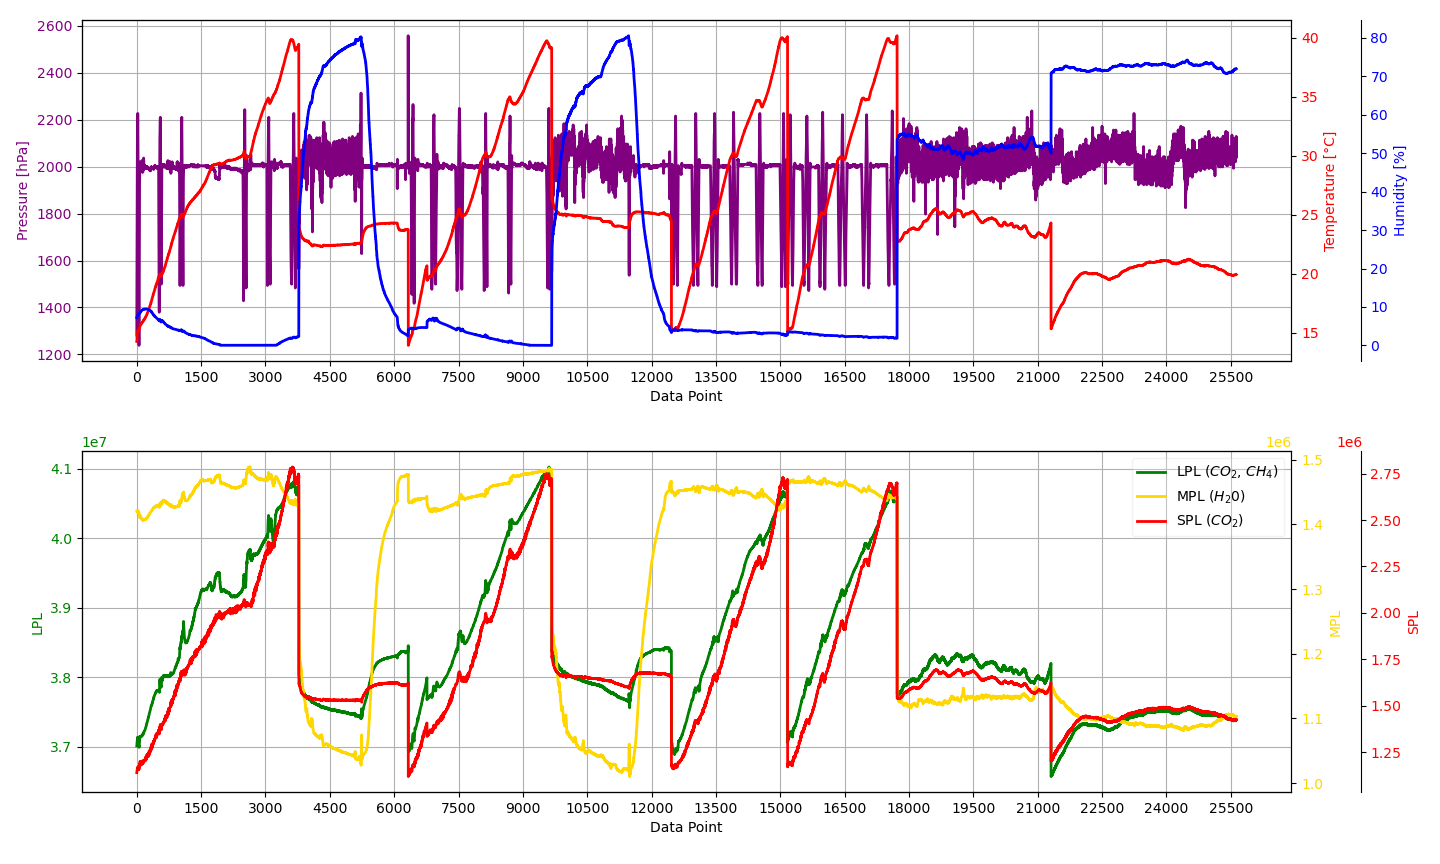
\includegraphics[width=1\linewidth]{figs/calibration/clean_data.png}
    \caption{Calibration dataset obtained in reference \cite{Olle2078608}.}
    \label{fig:calibration_data}
\end{figure}

The \textbf{calibration dataset} obtained in the study is presented in Figure \ref{fig:calibration_data}. For the dry data, were the humidity is somewhat constant and low, the molar fraction is varied with the lowest frequency, in steps. At each molar fraction step, the temperature is varied with a higher frequency, in steps. At each temperature step, the pressure is varied with the highest frequency. For the humid data, were the humidity reaches a peak and then decreases, the molar fraction is varied with the lowest frequency, in steps. At each molar fraction step, the humidity is varied, without the variation of temperature or pressure. For the reference instrument data, which is the last part of the dataset, no parameters are varied in steps.